% +--------------------------------------------------------------------+
% | Sample Chapter
% |
% | This file provides examples of how to
% | - insert a figure with a caption
% | - construct a table with a caption
% | - create subsections within the chapter
% | - insert a reference to a Figure or Table
% | - make a citation
% +--------------------------------------------------------------------+

\cleardoublepage

% +--------------------------------------------------------------------+
% | Replace "Chapter Title" below with the title of your chapter.  LaTeX
% | will automatically number the chapters.
% +--------------------------------------------------------------------+

\chapter{Introduction}
%\label{ch:Introducción}
\label{makereference}


% +--------------------------------------------------------------------+
% | Replace \section headings below with the title of your
% | subsections.  LaTeX will automatically number the subsections 1.1,
% | 1.2, 1.3, etc.
% +--------------------------------------------------------------------+

\section{Motivation}
\label{makereference1.1}

Cloud is a major word speaking about data compute in the last decade, we use cloud computing for processing every chunk of information from any source. 
If we move to Internet of Things field it is impossible not to put cloud computing in the same topic, cloud services are designed to provide easy, scalable access to applications, resources and services, and are fully managed by a cloud services provider.~\cite{cloud_def}  

Internet of things devices provide large amount of data, and we need cloud to process such kind of data, the Cloud of Things (CoT) term comes into play having devices connected directly to the cloud for perform complex operations with the generated data usually with Artificial Intelligence that is the perfect tool for creating smart tasks that would harness the immense amount of information.
However cloud computing now faces several challenges to meet the more stringent performance requirements of many applications services, specially in terms of latency and bandwith.~\cite{IEE:Morabito:2017}

To solve those problems, Edge computing is a new paradigm that aims to bring data storage and computation closer to a selected location in order to improve response times and save data bandwitch, this consist on increasing the resources available on the edge adopting a platform that provide intermediate layers.
Thinking about these layers located at the edge make impossible the idea of having the same kind of datacenter that are being used for Cloud computing, this layer implies limited computational capabilities so one of the main problems to solve is to get similar cloud platforms into an Edge environment with certain compute power for processing data.

\newpage
To solve this "compute power" problem the following resources are presented:
\begin{itemize}
  \item \textbf{Single Board computers or Minicomputers} that achieve high computing capacities reducing costs and size significantly.
  \item \textbf{Usb accelerators} devices that provides an Edge TPU as a coprocessor for your computer. It accelerates inferencing for artificial intelligence models.
\end{itemize}

Hardware part is covered, however there are too many things involving the current paradigm of cloud and edge computing that are essentials in order to build a proper architecture:

\textbf{Virtualization} is the capability of creating virtual machines that act like real ones, the creation of a virtual version of a device, this technology became mandatory in cloud and edge computing since the creation of automatic elastic services require to get rid of haphazard IT rooms, cables, and bulky hardware; reducing your overall IT overhead as well as management costs.~\cite{virt_def}.

Creation and management of these Virtual machines would be impossible without the existence of \textbf{hypervisors}, software which is responsible of controlling the virtual machine and provide a connection for the virtual resource and the real one.

\textbf{Virtual appliances} are Virtual Machine images, usually with a specific configuration, designed to run on a virtual platform. They are designed to reduce or eliminate the installation, configuration, and maintenance costs associated with running suites of software.~\cite{GEN:Virtualization:2010}

When anything would be able to connect to the Internet and generate data, there is a possibility that at some stage it is no longer necessary to upload the data to the cloud or sync device. Momentarily, the data may not be required. In that scenario, either the device must be stopped from generating data or gateway device must decide when it is required to stop uploading the data and not to consume resources of the network and cloud, for that while.~\cite{Ficloud:AazaamHuh:2014}
Having this in mind and knowing that in a near future there are going to be millions devices called things connected, the \textbf{IoT gateway} appears to serve as a bridge for connecting these things, send data to the cloud or participate with an edge approach, a way to implement this edge gateway might be build a virtual appliance that is situated close to the things. Figure ~\ref{figure1.1} show a representation of the concept.


\newpage
\begin{figure}[h]%t=top, b=bottom, h=here
% \centering
    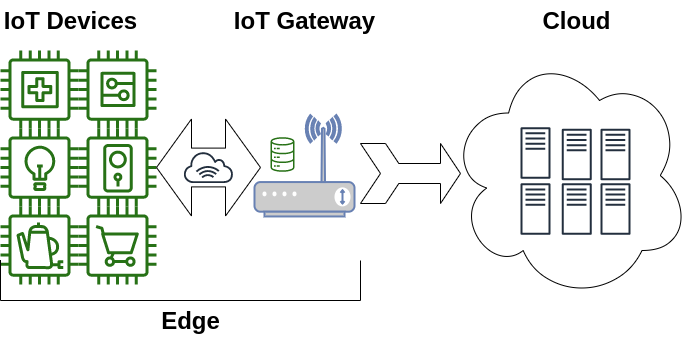
\includegraphics[width=6.5in]{figures/iot_gateway.png}
~\caption{IoT Gateway scheme}
\label{figure1.1}
\end{figure}

Some of the features that could supply the IoT gateway are the next:

\begin{itemize}
  \item communication bridge
  \item data storage, filter and aggregation
  \item device management and configuration
  \item Security 
  \item route data
\end{itemize}

The presence of this edge layer facilitate the implementation of collaborative computing among devices and it helps to apply data management policies, even so this edge layer is not usually resource enriched, following the cloud oriented approach of hypervisor-based virtualization can prove to be cumbersome on these devices.~\cite{arxiv:doluikiraly:2018}
However we'll see that this kind of approach could be very helpful using the proper hypervisor for gaining the maximum efficiency.

\newpage
\section{Objectives}
\label{makereference1.2}

This project has the main goal of prove that an IoT gateway using hypervisor-based virtualization reports improvements over an IoT edge environment providing virtual machines capable of use real USB accelerators connected through a low spec motherboard.

Therefore with the purpose of show some results, a virtual appliance has been created running a custom service developed entirely from scratch using new technologies, these areas are highlighted in greater detail in the next chapters. 

With our appliance working, the next milestones are going to be evaluated:

\begin{itemize}
  \item Inference with virtual machines using real USB accelerators
  \item The feature of share real USB accelerators between multiple virtual machines
  \item Dynamic resource allocation including CPU or memory 
\end{itemize}

\subsection{Use case}
\label{makereference1.2.1}
Under the principles previously established it has been defined a use case that allow the appliance development to have a concise scenario in order to achieve better results. The project is aimed at apartments block, takes into account a modern building in which every house can be considered smart home, having a large quantity of sensors across the property.

An external provider or a neighbourhood community want to take advantage of EpFiot we'll refer to that 'provider' as client:
\begin{itemize}
  \item A low cost board is deployed in base building of flats/apartments as an IoT Gateway with Epfiot appliance installed.
  \item Client provide each apartment with sensors (temperature, humidity, camera, gas...).
  \item Epfiot appliance has many GPU accelerators physically connected through usb ports.
  \item Epfiot appliance provide a service to the client allowing the spawn of customized vms that have direct access to the gpu accelerators.
  \item Client can configure sensors using epfiot.
  \item Client have full access and management for the vms and is able to allocate some resources including the usb accelerators.
  \item Sensors generate data, instead of send this data directly to internet, a proper vm could receive the data and use a accelerator for perform inference.
  \item Results could be stored in epfiot or another application in a low latency context.
\end{itemize}

Figure ~\ref{figure1.2} shows a representation of the case listed above.

\begin{figure}[h]%t=top, b=bottom, h=here
% \centering
    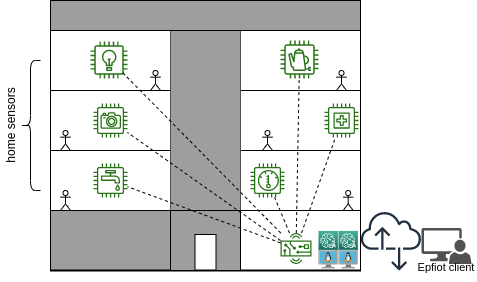
\includegraphics[width=6.5in]{figures/use_case.png}
~\caption{epfiot use case example}
\label{figure1.2}
\end{figure}

\newpage
\section{Document Organization}
\label{makereference1.3}

The work is formed by seven chapters, we shall now proceed to enumerate these chapters:

\begin{itemize}
  \item \textbf{Chapter 1, Introduction:} This chapter introduces a set of conceptual definition that are going to be mentioned along the document, also this chapter shows the purpose of the whole project explaining motivations and goals.
  \item \textbf{Chapter 2, State of the Arts:} This section shows the current state of Edge computing from a infrastructure point of view, discussing the underlying technologies discussing advantages and disadvantages of each option, finally a brief overview of related projects are shown.    
  \item \textbf{Chapter 3, Development Environment:} A list of the main technologies used for Epfiot will be enumerated, underlining what kind of utility provide to the project. Hardware and requirements are also discussed in this chapter.
  \item \textbf{Chapter 4: Architecture}: The chapter describe the overall architecture of Epfiot, reviewing every component and how they are connected between each other. 
  \item \textbf{Chapter 5: Features:} This part explains with detail the features of the project, end-user's functionalities are listed.   
  \item \textbf{Chapter 6: Results:} This section is about showing the final results that are obtained with the Epfiot application running. 
  \item \textbf{Chapter 7: Conclusions and Future Work:} Finally a brief summary of the work commenting what kind of implications and how to improve the current status of the project in a near future. 
\end{itemize}

%Here's an example of a citation to a single
%work.~\citet{CT:Weiner:1999} It's also possible to make multiple
%citations.~\citet{CT:Phillips:1985, ARP:Loy:1974}
